\section{Introduction}

Information Extraction (IE) is a fundamental task in Natural Language Processing (NLP), which aims to extract structured information from unstructured text, such as Named Entity Recognition (NER), Relation Extraction (RE), Event Extraction (EE), etc.
Each IE task is usually isolated, and it needs specific datasets and delicate models, which makes it difficult to build complex applications.
It is a fascinating problem to combine different IE tasks into a whole, and make one model for universal IE tasks.

There are two ways to combine different IE tasks.
The first is to utilize generative pretrained language models (PLMs) to generate the structured information directly.
x, x and x structure the IE tasks as a sequence generation problem, and use T5 models to predict the structured information autoregressively.
However, such methods cannot provide the exact positions of the structured information, which is important for some IE tasks, such as NER.
Besides, the generation-based methods are usually slow, and it is difficult to train them on large-scale datasets.
The second is to apply the extractive PLMs, which is way more faster to train and inference.
UIE unifies the IE tasks into span spotting and associating problems.
Based on this idea, x, x and x take the IE tasks into a triplet prediction problems, and propose different methods.
However, such methods are not suitable for multi-span and n-ary IE tasks.

\begin{figure}[t]
    \centering
    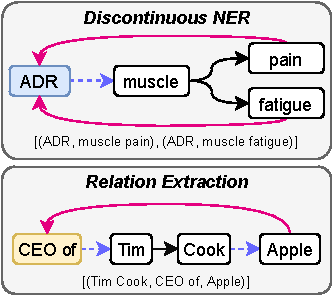
\includegraphics[width=\columnwidth]{figs/Multi-span Cyclic Graph.pdf}
    \caption{
        Multi-span cyclic graph for discontinuous NER and RE tasks (best viewed in color).
        The spans are connected by three types of edges, including \textbf{\textit{consecutive connections}}, dotted \textbf{\color[HTML]{695efb} \textit{jump connections}} and \textbf{\color[HTML]{E9087F} \textit{tail-to-head connections}}.
        \textit{ADR} in discontinuous NER denotes the entity label of Adverse Drug Reaction.
    }
    \label{fig:multi-span-cyclic-graph}
\end{figure}

\begin{table*}[t]
    \centering
    \resizebox{\textwidth}{!}{%
        \begin{tabular}{c|ccccccc|c}
        \toprule
        Model & TANL & UIE & DeepStruct & InstructUIE & USM & UniEX & RexUIE & Mirror \\
        \midrule
        PLM & T5-base & T5-large & GLM & FlanT5 & RoBERTa & RoBERTa & DeBERTa-v3 & DeBERTa-v3 \\
        \#Params & 220M & 770M & 10B & 11B & large 372M & large 372M & large 434M & large 434M \\
        \midrule
        Single-step & {\color[HTML]{008114}\cmark}    & {\color[HTML]{008114}\cmark}   & {\color[HTML]{008114}\cmark}          & {\color[HTML]{008114}\cmark}           & {\color[HTML]{008114}\cmark}   & {\color[HTML]{008114}\cmark}     & \textcolor{red}{\xmark}      & {\color[HTML]{008114}\cmark}      \\
        Indexing & \textcolor{red}{\xmark} & \textcolor{red}{\xmark} & \textcolor{red}{\xmark} & \textcolor{red}{\xmark} & {\color[HTML]{008114}\cmark} & {\color[HTML]{008114}\cmark} & {\color[HTML]{008114}\cmark} & {\color[HTML]{008114}\cmark} \\
        NAR         & \textcolor{red}{\xmark}    & \textcolor{red}{\xmark}   & \textcolor{red}{\xmark}          & \textcolor{red}{\xmark}           & {\color[HTML]{008114}\cmark}   & {\color[HTML]{008114}\cmark}     & {\color[HTML]{008114}\cmark}      & {\color[HTML]{008114}\cmark}      \\
        Multi-span  & \textcolor{red}{\xmark}    & $\circ$    & $\circ$           & $\circ$            & \textcolor{red}{\xmark}   & \textcolor{red}{\xmark}     & \textcolor{red}{\xmark}      & {\color[HTML]{008114}\cmark}      \\
        N-ary       & \textcolor{red}{\xmark}    & \textcolor{red}{\xmark}   & \textcolor{red}{\xmark}          & \textcolor{red}{\xmark}           & \textcolor{red}{\xmark}   & \textcolor{red}{\xmark}     & {\color[HTML]{008114}\cmark}      & {\color[HTML]{008114}\cmark} \\
        \bottomrule
        \end{tabular}
    }
    \caption{
        Comparisons with other systems.
        Single-step represents that the model predicts results in a single step.
        Indexing means whether the model could provide exact information positions.
        NAR denotes the non-autoregressive decoding strategy.
        Multi-span means the model supports multi-span extraction, e.g. the discontinuous named entity recognition task.
        N-ary denotes the ability of n-ary tuple extraction.
        $\circ$ means the model supports the task theoretically, but the implementation is not available.
    }
    \label{tab:method_comparison}
\end{table*}

To extend the universal IE systems into more tasks, we propose a multi-task framework, namely Mirror, which can be applied on various IE tasks, including multi-span and n-ary extraction problems.
We formulate IE tasks into a unified schema-guided multi-span graph, and regard labels as spans' leading tokens.
We design three kind of connections and utilize the biaffine-style method to extract the structured information.

% how well did we do it
We conduct extensive experiments on 6 IE tasks, including NER, RE, EE, Aspect-based Sentiment Analysis (ABSA), multi-span discontinuous NER and n-ary hyper RE.
Our Mirror shows good compatibility across different tasks and datasets, and achieves competitive results on few-shot settings.
Besides, 434M Mirror outperforms FlanT5-11B InstructUIE in zero-shot NER tasks.

% contribution
Our contributions are summarized as follows:
\begin{itemize}
    \item We propose a multi-task framework, namely Mirror, which can be trained on various IE tasks, including multi-span and n-ary extraction problems.
    \item We conduct extensive experiments on x IE tasks, and the results show that our model achieves state-of-the-art performance on most of the tasks.
\end{itemize}
